\begin{frame}{Practice!}
    \begin{columns}[onlytextwidth]
        \begin{column}{0.5\textwidth}
            Implement the 1-dimensional version of
            \begin{itemize}
                \item Gradient Descent
                \item Basic SGD
            \end{itemize}
            Then compare convergence of the two algorithms on one or both test functions
            $$f_1(x) = 3(x - 3)^2 - 1 \quad \text{and} \quad f_2(x) = (x - 1)^3 - 4x^2 + 4$$

            Also vary the initial guess $x_0$ and the learning rate $\eta$. What happens 
            e.g. for $f_2$ with $x_0 = 0$?
        \end{column}
        \begin{column}{0.5\textwidth}
            \centering
            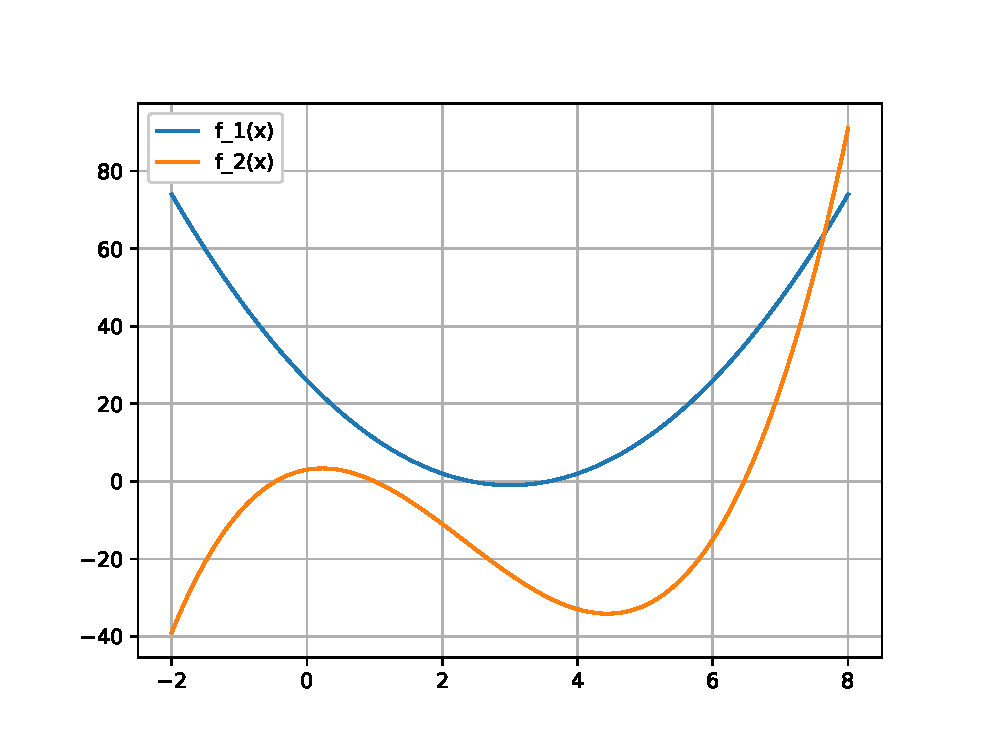
\includegraphics[width=\textwidth]{fig/ex_polys.eps}
        \end{column}
    \end{columns}
\end{frame}

% Python code to generate figure
% f = lambda x: 3*(x - 3)**2 - 1
% xs = np.linspace(-2, 8, 100)
% plt.plot(xs, [f(x) for x in xs])
% f = lambda x: (x - 1)**3 - 4*x**2 + 4
% plt.plot(xs, [f(x) for x in xs])
% plt.grid(True)
% plt.legend(['f_1(x)', 'f_2(x)'])
% plt.show()
